\documentclass[11pt, oneside, a4paper]{report}   %11pt font, one sided, A4, UK English
\usepackage [autostyle]{csquotes} %Fixes Quotation marks
\MakeOuterQuote{"} %Required for csquotes
\usepackage[utf8]{inputenc} %UTF-8 Encoding
\usepackage[colorlinks=true,urlcolor=magenta, linkcolor=red]{hyperref} %Colours links instead of highlighting with a box, URL's are Magenta
\usepackage{minitoc-hyper} %Used to give contents pages for individual chapters. Mini Tables of Contents.

%Put "DRAFT" in the background.  Due to Filox
\usepackage{graphicx} %or \usepackage{graphicx}
\usepackage{type1cm}
\usepackage{eso-pic}
\makeatletter
\AddToShipoutPicture{ %
	\setlength{\@tempdimb}{.5\paperwidth}%
	\setlength{\@tempdimc}{.5\paperheight}%
	\setlength{\unitlength}{1pt}%
	\put(\strip@pt\@tempdimb,\strip@pt\@tempdimc){ %
		\makebox(0,0){\rotatebox{55}{\textcolor[gray]{0.95} %
				{\fontsize{7cm}{7cm}\selectfont{DRAFT}}}}%
		% Adjust 7cm to desired font size as necessary
	} %
}
\makeatother

\begin{document}
\dominitoc %Initialises the Domain of the MiniTOC
\chapter{Project Evaluation} 
\pagebreak
\minitoc
\pagebreak
\section{Organisation} \label{sec:Organisation}
\subsection{"How was your group organised? Was it successful?"} \label{sec:Organisation - 1}

The organisation of Buzzword varied dramatically during the three distinct stages of the project:  \\ \\
At Stage One the group worked in small teams of two or three to complete a delegated section of the 
specification document each: this was determined by the Organisational Manager and was 
determined to be the best course of action for the project at this particular time as, since each section awarded 
relative autonomy (e.g. The Requirements Analysis does not depend on the Risk Analysis and vice versa), groups 
could organise themselves easier with less people which, in theory, would have reduced the overhead of working as a team. \\ \\
At Stage Two, the group was split into a "Core Dev" team and a "Web" team containing three people each and with the Organisational
Manager being involved in both teams. The idea here was that one team would focus all its efforts on the Company Website and subsequent 
branding etc. while the other team focused on developing the main application; the Organisational manager would help out where possible 
then handle the Progress Report section. Much like Stage One, the core motivation was to reduce the burden of "people management" and 
allow teams to organise themselves with a better focus on what is important to them with less conflict of schedules being awarded by having less
people.\\ \\
At Stage Three, the group took on a hybrid organisation of Stages One and Two: the "Core Dev" team remained as a small team but gained one
member from the "Web" team, while the "Web" team disbanded into two separate individuals who could on the tasks of the "Marketing Analysis and Strategy"
and, once the application was complete, the " Final Usability Evaluation" without relying on anyone else. Like the previous two organisational methods 
the strategy was very much to split the work into distinct sections people could work on without relying on others and this was true throughout the whole project.\\ 

It is the view of Buzzword that this approach was ill-thought-out and poorly adhered to. While the "divide and concur" nature of the approach could have the 
opportunity to be successful; more frequent, whole group and team, meetings would have greatly aided the project's progress. 
As everyone was, for the most part, able to work on a section independently there was miscommunication about the intended overview of the system and 
implementation strategy, and while we did mange to produce a functioning application the end product could have been greatly improved by more 
frequent reporting from each member to the rest of their team, the group as a whole, and to the Organisational Manager as well as the group manager.\\ 
In any theoretical future projects, we would aim to have daily standup "SCRUM" meetings for each of the teams, as well as a weekly meeting where each member
can report on their progress to the rest of the group, as well as the Organisational Manager, and the group manager.  
\subsection{"How well did your group collaborate? How did you handle any problems which arose?"} \label{sec:Organisation - 2}
We made a reasonable attempt to collaborate well, but due to the organisational strategy outlined above this was largely not required from the group. Very few sections, 
with the exception of cross communication of the components in the "Core Dev" team required members to be dependant on others/work on the same document 
together. That being said, there was a positive "team sprit" with reasonable turnout during group meetings and only one member absent without explanation during during
the Stage Two demonstration to the group manager. Thought the project, limited problems arose due to the organisational strategy however;  there were bereavements from 
certain members resulting in delays to their sections of work, as well as difficulties with group meetings during the period of industrial action experienced by Heriot-Watt University.
The former was handled by simply accepting and accounting for the delays that were inevitable, and the former was handled by working to the best of our ability independently and 
communicating via a group chat.
\subsection{"How successful were the timings in your original plan?"} \label{sec:Organisation - 3}
Not at all. From Week One of the original implementation plan the organisation and structure of the SCRUM methodology of which the plan was based around was immediately 
abandoned. The group intended to get "back on plan" but the disruption to ordinary working schedules awarded by examinations and the holiday period were not suitably accounted 
for in the plan. As such, by the time the holidays were over and normality had returned the group were so far off track that it was no longer practical to attempt to follow the plan 
which had been originally outlined. An "ad-lib" approach was taken to planning for the rest of the project prioritising must have functional requirements, and sections which were most
urgently due. 
\pagebreak
\section{Implementation}
\textit{It is assumed that "Implementation" here refers solely to the coding and development of the application and not the implementation of the project as a whole}
\subsection{"What was your implementation schedule and how did this differ from the original plan?"} \label{sec:Implementation - 1}
Our implementation schedule consisted of a short burst at the start of Stage Two where the server was implemented, followed by a hiatus until shortly before the Stage Two deadline, followed by a short burst where some 
functionality of each of the components was implemented, followed by another hiatus until shortly before the Stage Three deadline, followed by a short burst where the remaining application was developed. Exact timings 
and what was accomplished when can be obtained by viewing the commit history of the project's GitHub repository in the Appendix. This differed immensely from the original plan of frequent and gradual development of
each of the requirements as opposed to the bursts experienced. 
\subsection{"Was your implementation approach successful (e.g., SCRUM, other agile, etc.)? Why or why
not?"} \label{sec:Implementation - 2}
It could be argued that our implementation approach was not unsuccessful with a reasonable product being developed and delivered at the end of the project. However, this comes with the significant caveat that we did not 
achieve everything we had planned, and the end product was not of as high quality as we would have liked. The group feels the implementation approach, therefore, was unsuccessful but this was not a result of the planned 
implementation methodology adopted but rather that it was not adhered to at all.  
\subsection{"Which languages, tools, and techniques did you use? How suitable were they?"} \label{sec:Implementation - 3}
%TODO: Tommy
\pagebreak
\section{Product} 
A most of the core functionality required by the specification document has been implemented. A notable omission is the inclusion of the ability for a waiter to amend an existing order; this has cascading consequences where a number of our "Could Have" or "Should Have" requirements were not implemented as these related to the amendment of orders. 
\subsection{"How many of your requirements did you meet?"}
The table below references our Stage One - The Bid document and outlines each of the Functional Requirements with indications of the degree to which each of these were implemented.\\

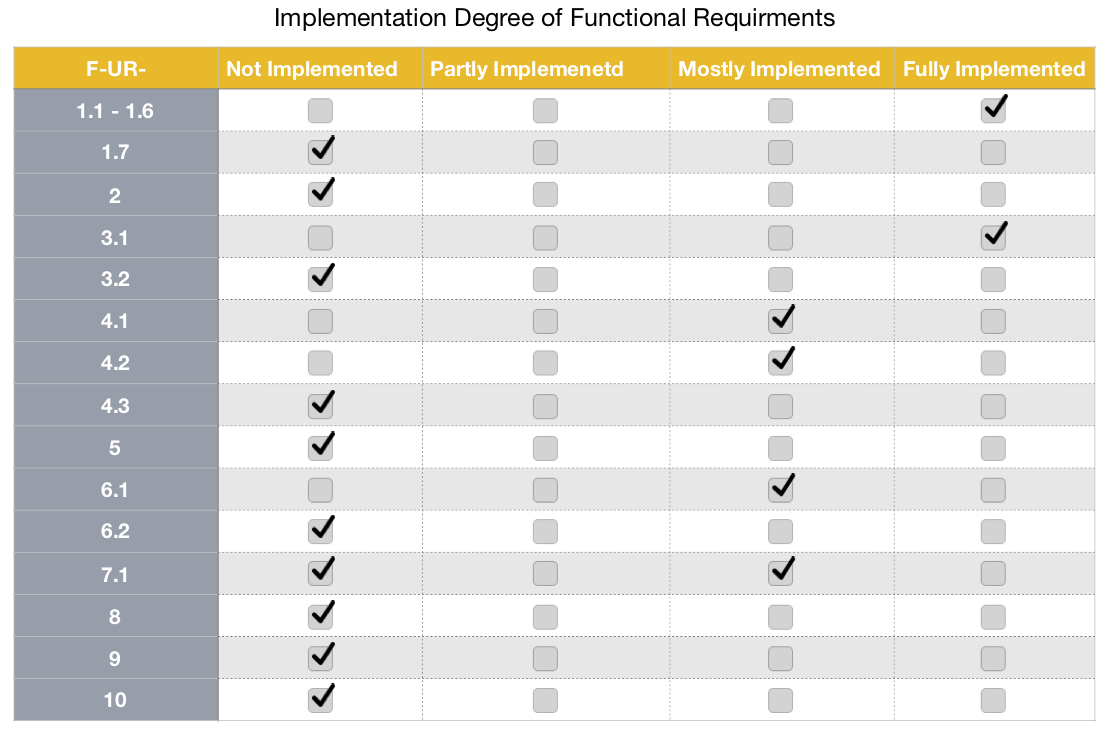
\includegraphics[width=\textwidth]{FR}

\subsection{"What is particularly special about your product? Have you included extra features?"}
The key selling point of our application is the ability to perform the requested functionality without the need for either the customer or the waiter to have/create an account. We felt that account creation would be cumbersome for the user and as such deliberately avoided it. No extra features have been included outside of what was outlined in our original requirements document. 
\subsection{"How robust is your final system? Are there known bugs or constraints?"}

The resulting system is fairly robust with only one known bug, that being that the server does not check for the correctness of any JSON it returns. This could, in theory, result in unpredictable system behaviour in the future. However, there are a number of constraints with the system but these all relate to the unimplemented functionality discussed previously.
\subsection{"How usable did your subjects find the final system?"}
%TODO:Kerr
\end{document}  